\section{Introduction}
\label{sec:introduction}

A full-duplex conversational assistant must continue processing input while speaking so that it can respond to interruptions.
MiniCPM-o 4.5, for example, processes input in one-second chunks and decides in each chunk whether to speak~\cite{cui2026minicpmo45}.
Following Thinking Machines Lab, we call these short interaction intervals \emph{micro-turns}~\cite{thinkingmachines2026interactionmodels}.
The model incorporates new input and generates output when needed, reusing history from earlier micro-turns.
Serving many such sessions requires managing both their recurring computation and the state that persists between updates.

The memory cost of this state grows with the retained history.
Models cache attention keys and values (KV) so that later micro-turns can reuse previously processed history.
For MiniCPM-o 4.5, ten minutes of retained input audio alone corresponds to approximately 0.82\,GiB of KV per session in BF16.
This estimate follows from the model's 10 audio feature tokens per second and 144\,KiB of KV per backbone position~\cite{cui2026minicpmo45,openbmb2026minicpmconfig}.
It is a calculation from published parameters, with full retention assumed; it excludes text, visual inputs, control tokens, other model state, and allocation overhead.
% 2 (K and V) * 36 layers * 8 KV heads * 128 dimensions * 2 bytes = 144 KiB/position.
% 10 positions/s * 600 s * 144 KiB/position = 0.823974609375 GiB.

Full residency keeps this KV on the GPU even after a micro-turn finishes, when the state is idle until the next update (Figure~\ref{fig:motivation}).
As histories grow, their combined KV can fill the available memory while all admitted sessions' work still leaves time within each period.
This condition concerns the whole GPU: an individual session's idle interval may be occupied by another session's computation.
We focus on configurations where KV capacity limits concurrency before the aggregate execution budget is exhausted.

\begin{figure*}[t]
  \centering
  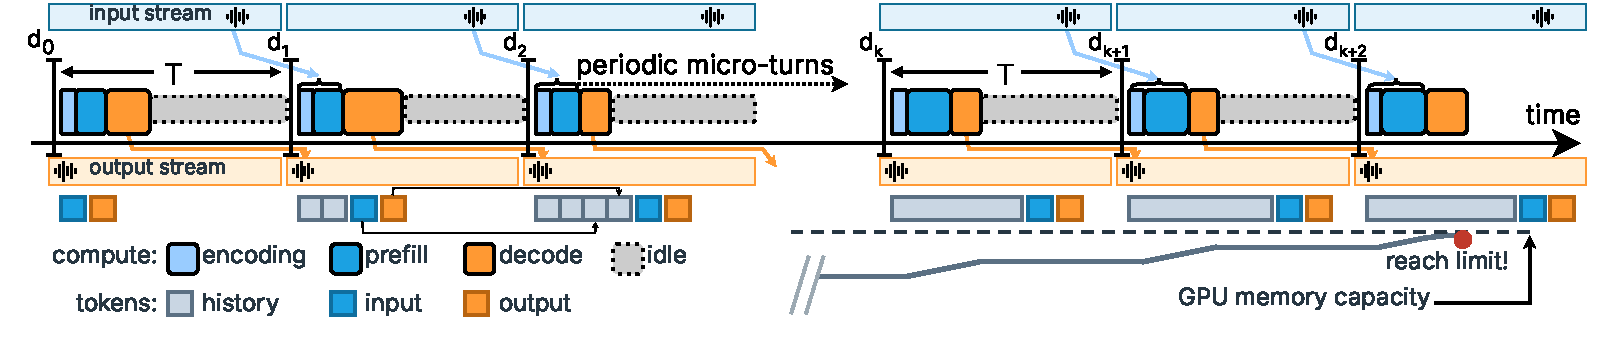
\includegraphics[width=\linewidth]{figures/figure-intro.pdf}
  \caption{Periodic execution with persistent history.
  Each micro-turn encodes and prefills new input and may decode output for playback.
  Retained input and output extend the KV history, which occupies GPU memory even between micro-turns under full residency.
  The timeline and memory growth are schematic, illustrating how retained state can reach the capacity limit.}
  \label{fig:motivation}
  \Description{A periodic session processes input, generates output, and waits for the next period.
  Its retained token history grows, and the corresponding illustrative KV footprint reaches a GPU capacity line.}
\end{figure*}

Retaining less history and offloading idle state make different tradeoffs.
Metronome bounds the KV window of periodic sessions and uses deadline feedback to control admission~\cite{meng2026metronome}.
When an application needs a longer history, offloading idle KV to host memory preserves that history but requires recovery before its next use.
InferCept, for example, chooses among retaining, swapping, and recomputing state for requests paused by external interactions~\cite{abhyankar2024infercept}.
In periodic service, eviction between micro-turns makes recovery a recurring obligation.
Restoring KV only when the next micro-turn arrives delays that micro-turn's computation (Figure~\ref{fig:comparison}(a)).

Periodic execution provides advance notice of when state will be needed again.
The start of each period, or \emph{tick}, is known, so restoration can be scheduled before the next micro-turn.
If the application permits phase assignment, the server can also choose each session's start offset within the period.
Staggering these starts creates opportunities for sessions to reuse GPU space as their state becomes idle.
We call this reuse \emph{memory multiplexing}: each session retains its own history, but its KV need not occupy GPU space throughout the period.

The difficulty is that restoration itself consumes the space that eviction releases.
The server must allocate the entire destination before a copy begins, although the restored KV becomes usable only after the copy finishes.
An early restoration therefore occupies memory that other sessions may still need; a later one has less time to finish before the next tick.
Evicting more KV also increases the time needed to restore it.
The question is how to coordinate session phases, eviction amounts, and restoration times so that transfers finish when needed without exceeding GPU capacity.

\begin{figure}[t]
  \centering
  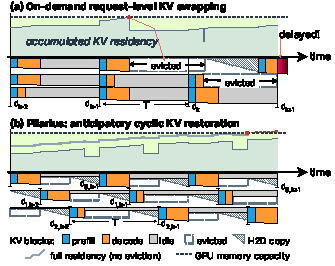
\includegraphics[width=\linewidth]{figures/figure-comparison.pdf}
  \caption{Schematic comparison of restoration timing.
  (a) On-demand swapping delays computation until KV returns.
  (b) Staggered sessions release space for one another's restorations before their next ticks.
  Upper curves show aggregate GPU KV allocation, including each restoration's full destination from the start of allocation.
  Hatching denotes host-to-device (H2D) copies, dotted outlines denote evicted state, and gray denotes idle resident KV.
  The pale curve in (b) shows full residency.}
  \label{fig:comparison}
  \Description{On-demand restoration delays a session, whereas staggered sessions alternate eviction and restoration before their next ticks.
  Aggregate GPU allocation includes the full destination of each ongoing H2D copy.
  A pale curve shows the higher allocation under full residency.}
\end{figure}

We present \systemname, a design for memory multiplexing through \emph{cyclic KV restoration}.
After a micro-turn, \systemname evicts part of the session's idle KV and schedules its restoration to finish by the next tick.
It coordinates these operations across staggered sessions, arranging for space released by one session to accommodate another's restoration (Figure~\ref{fig:comparison}(b)).
The design accounts for both the shared transfer schedule and the GPU space available for each restoration.
Its goal is to increase concurrency while preserving retained history and meeting a recurring soft deadline: each micro-turn should finish by the next tick.

Continued history growth requires planning beyond the current period.
At admission, \systemname considers expected KV growth, computation, transfers, and GPU allocation over a finite lookahead interval.
The resulting plan is reused across micro-turns and revised infrequently as histories grow or sessions enter and leave.
This planning anticipates changes in resource demand; feasibility within the lookahead interval does not guarantee capacity for an entire session.

\placeholder{Final contributions and measured results: identify the configurations where KV capacity limits concurrency while compute time remains; establish the benefit attributable to coordinating phases, eviction amounts, and restoration timing; report concurrency and deadline-miss rates against full residency and on-demand restoration under matched service objectives.}
